\documentclass[11pt,a4paper]{article}

\newcommand{\tumsoTime}{09:00 น. - 12:00 น.}
\newcommand{\tumsoRound}{1}

\usepackage{../tumso}

\begin{document}

\begin{problem}{Isekai No Hajime}{standard input}{standard output}{1 seconds}{256 megabytes}{100}

“ยินดีต้อนรับ ผู้กล้าจากต่างโลก!”\\*
อะไรกัน! นี่ฉันกำลังนั่งรถไฟเพื่อจะมาเข้าร่วมการแข่งขันการเขียนโปรแกรมไม่ใช่หรอ?!\\*
“ข้าคือราชาแห่งจักรวรรดิ $Lomak$ ท่านจงช่วยเราด้วยเถิด ขณะนี้โลกของเราอยู่ในภาวะวิกฤตแล้ว!”\\*
ไม่มีทางหรอกท่านราชา-- เดี๋ยวก่อน! นั่นใครน่ะ ..ช่างน่ารักซะเหลือเกิน..\\*
“ท..ท่านผู้กล้า อย่าจ้องข้ามากสิ"\\*
"โฮ่ นี่ท่านสนใจองค์หญิงขนาดนั้นเลยหรอ ได้เลย หากท่านช่วยเหลือเราสำเร็จ ข้าจะมอบนางให้ท่าน ข้าก็รู้ว่าตัวนางเองก็สนใจในตัวท่านมาตั้งแต่แร--"\\*
"ท่านพ่อ!"\\*
องค์หญิงมีท่าทางเขินอาย.. น่ารักจังงง\\*
"ถ้าอย่างนั้น กระผมขอน้อมรับโดยดีครับ!"\\*
"เอาล่ะ นี่บัตรผจญภัยของท่าน $\#11095$ ผู้กล้าหนึ่งเดียวของเรา"\\

สำหรับการต่อสู้ของเรา สนามรบของเรานับว่าเป็นสองมิติ (ยาว×สูง) มีความยาว $N$ กิโลเมตร ซึ่งทุกๆกิโลเมตรที่ $i$ จะมีความสูง $L_i$\par
ฝั่งมนุษย์เรา มีปืนใหญ่ยักษ์ขนาด $1$ ถึง $M$ กิโลเมตร ซึ่งแต่ละกระบอกก็มีความแรง (ดาเมจ) ต่างๆกัน ปืนที่ยาว $j$ จะมีความแรง $DMG_j$ หน่วย และด้วยเทคโนโลยีของโลกนี้ \textbf{ปืนใหญ่จะสามารถถูกติดตั้งได้เฉพาะบนระนาบที่มีความยาว $j$ พอดีเท่านั้น} \par
เรามีเวลา $P$ วันก่อนที่ราชาปีศาจจะทำลายเมืองลง อย่างไรก็ตาม ทุกๆคืน คืนที่ $k$ ราชาปีศาจจะยิงลำแสงเลเซอร์ทำลายล้างที่ระดับ $H_k$ ซึ่งด้วยความโหดของเขา ทุกๆสิ่งที่อยู่เหนือแนวนั้นสูงขึ้นไปจะกลายเป็นฝุ่นไป \textbf{โดยบริเวณที่ถูกทำลายหายไปไม่เต็มช่วงกิโลเมตร เราถือว่าส่วนนั้นไม่สามารถวางปืนใหญ่ได้}\par
เราไม่ทราบพลังชีวิตอันมหาศาลของราชาปีศาจอย่างชัดเจน แต่หน่วยสอดแนมคาดคะเนไว้ $Q$ ค่า นั่นคือ $HP_l$ ในการคาดที่ $l$\par
ในช่วงกลางวันของทุกๆวัน เราสามารถตั้งปืนใหญ่กี่กระบอกก็ได้และยิงได้กระบอกละหนึ่งครั้งก่อนที่จะตกดึก (ไม่มีเวลาเก็บ) ด้วยความร่ำรวยของราชาแห่ง $Lomak$ เราถือว่าปืนใหญ่และกระสุนของทุกกระบอกมีจำนวนไม่จำกัด แต่ปืนใหญ่ยิงได้เพียงในแนวระนาบบนสุดของสนามรบในขณะนั้นเท่านั้น จะยิงโดนราชาปีศาจทุกนัด และจะไม่ยิงโดนกันเอง \\
เพื่อที่จะรีบมาพบกับองค์หญิง ผู้กล้าต้องการทราบว่า พลังชีวิตของราชาปีศาจจะหมดไวที่สุดได้ในคืนที่เท่าไหร่ โดยถือว่าการรบเริ่มที่คืนแรกที่ราชาปีศาจยิงเลเซอร์

\InputFile
บรรทัดที่ $1$ รับจำนวนเต็ม 4 จำนวน: $N$ $M$ $P$ และ $Q$ // ขนาดสนาม จำนวนปืน จำนวนคืน จำนวนการคาดคะเนพลังชีวิต

บรรทัดที่ $2$ รับจำนวนเต็ม $N$ จำนวน: $L_i$ // ความสูงของพื้นแต่ละจุด

บรรทัดที่ $3$ รับจำนวนเต็ม $M$ จำนวน: $DMG_j$ // ความแรงของปืนแต่ละกระบอก

บรรทัดที่ $4$ รับจำนวนเต็ม $P$ จำนวน: $H_k$ // ระดับของเลเซอร์แต่ละคืน

บรรทัดที่ $5$ รับจำนวนเต็ม $Q$ จำนวน: $HP_l$ // พลังชีวิตของราชาปีศาจที่คาดคะเนไว้แต่ละค่า

\OutputFile
มี $Q$ ค่า นั่นคือจำนวนคืนที่ไวที่สุดที่จะฆ่าราชาปีศาจตามค่าคาดคะเนของพลังชีวิตแต่ละค่า

หากไม่สามารถฆ่าราชาปีศาจได้ภายใน $P$ วัน ให้ตอบ $-1$

\section*{Constraints}

$1 \leq N,$ $M,$ $P,$ $Q \leq 200,000$

$1 \leq L_i,$ $DMG_j,$ $H_k,$ $HP_l \leq 2,000,000,000$
  
\Scoring
ชุดทดสอบจะถูกแบ่งเป็น 2 ชุด จะได้คะแนนในแต่ละชุดก็ต่อเมื่อโปรแกรมให้ผลลัพธ์ถูกต้องในชุดทดสอบย่อยทั้งหมด

\begin{description}

\item[ชุดที่ 1 (15 คะแนน)]  $1 \leq N,$ $M,$ $P,$ $Q \leq 2,000$ 

\item[ชุดที่ 2 (25 คะแนน)]  $1 \leq L_i,$ $DMG_j,$ $H_k,$ $HP_l \leq 2,000,000$

\item[ชุดที่ 3 (60 คะแนน)] ไม่มีเงื่อนไขเพิ่มเติม

\end{description}

\Examples

\begin{example}
\exmp{11 3 5 4
5 2 3 1 7 1 3 4 4 6 2
1 2 3
4 6 4 3 2
5 7 11 12
}{3 4 5 -1
}%
\exmp{11 4 6 6 
5 2 3 1 7 1 3 4 4 6 2
3 3 1 1
4 5 3 4 2 2
11 8 9 15 17 6
}{5 4 5 6 -1 2
}%
\end{example}

\section*{คำอธิบายตัวอย่างที่ 1}
หากราชาปีศาจมีพลังชีวิต $5$ เราสามารถฆ่ามันได้ด้วยปืนใหญ่ยาว $2$ ดาเมจ $2$ โดยวางที่ตำแหน่ง $7 - 9$ ยิง $3$ ครั้ง

หากราชาปีศาจมีพลังชีวิต $7$ สามคืนแรกเรายิงเหมือนเคสที่แล้ว ($6$ ดาเมจ) และในคืนที่ $4$ เรายิงด้วยปืนใหญ่ยาว $3$ ดาเมจ $3$ ตำแหน่ง $6 - 9$

หากราชาปีศาจมีพลังชีวิต $11$ สี่คืนแรกเรายิงตามเตวสอง $9$ ดาเมจ คืนที่ $5$ เรายิง ที่ตำแหน่ง $0 - 2$ อีก $2$ ดาเมจ

หากราชาปีศาจมีพลังชีวิต $12$ เราไม่สามารถฆ่าได้ภายใน $5$ คืนนี้

\textit{สังเกตว่าเราวางปืนที่ตำแหน่ง $6 - 10$ ไม่ได้เพราะไม่มีปืนขนาด $4$}

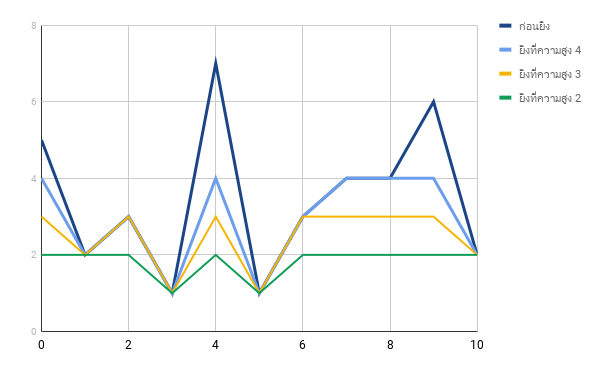
\includegraphics[width=\textwidth]{chart.png}

\end{problem}

\end{document}
